\documentclass{article}
%\usepackage[T1]{fontenc}
%\usepackage{amssymb, amsmath, graphicx, subfigure, enumerate}
%\usepackage{amsthm,alltt} 
\usepackage[margin=1.25in]{geometry} %geometry (sets margin) and other useful packages
\usepackage{graphicx,ctable,booktabs}
\usepackage{mathtools}
\usepackage[boxed]{algorithm2e}
\usepackage{mathdots}
\usepackage{fancyhdr} %Fancy-header package to modify header/page numbering
\usepackage{cleveref}

\setlength{\oddsidemargin}{.25in}
\setlength{\evensidemargin}{.25in}
\setlength{\textwidth}{6in}
\setlength{\topmargin}{-0.4in}
\setlength{\textheight}{8.5in}



\newcommand{\heading}[6]{
  \renewcommand{\thepage}{\arabic{page}} % used to be #1-\arabic{page}
  \noindent
  \begin{center}
  \framebox{
    \vbox{
      \hbox to 5.78in { \textbf{#2} \hfill #3 }
      \vspace{4mm}
      \hbox to 5.78in { {\Large \hfill #6  \hfill} }
      \vspace{2mm}
      \hbox to 5.78in { \textit{{Name: }} }
    }
  }
  \end{center}
  \vspace*{4mm}
}

%Redefining sections as problems
\makeatletter
\newenvironment{problem}{\@startsection
       {section}
       {2}
       {-.2em}
       {-3.5ex plus -1ex minus -.2ex}
       {2.3ex plus .2ex}
       {\pagebreak[3]%forces pagebreak when space is small; use \eject for better results
       \large\bf\noindent{Problem }
       }
       }
       %{%\vspace{1ex}\begin{center} \rule{0.3\linewidth}{.3pt}\end{center}}
       %\begin{center}\large\bf \ldots\ldots\ldots\end{center}}
\makeatother


\newtheorem{theorem}{Theorem}[section]
\newtheorem{definition}[theorem]{Definition}
\newtheorem{remark}[theorem]{Remark}
\newtheorem{lemma}[theorem]{Lemma}
\newtheorem{corollary}[theorem]{Corollary}
\newtheorem{proposition}[theorem]{Proposition}
\newtheorem{claim}[theorem]{Claim}
\newtheorem{observation}[theorem]{Observation}
\newtheorem{fact}[theorem]{Fact}
\newtheorem{assumption}[theorem]{Assumption}

%\newenvironment{proof}{\noindent{\bf Proof:} \hspace*{1mm}}{
% \hspace*{\fill} $\Box$ }
%\newenvironment{proof_of}[1]{\noindent {\bf Proof of #1:}
% \hspace*{1mm}}{\hspace*{\fill} $\Box$ }
%\newenvironment{proof_claim}{\begin{quotation} \noindent}{
% \hspace*{\fill} $\diamond$ \end{quotation}}

\newcommand{\problemset}[3]{\heading{#1}{\classname}{#2}{\studentname}{#3}{Problem Set #1}} % Don't change this line
%%%%%%%%%%%%%%%%%%%%%%%%%% Change this stuff below, don't change the line above this one
\newcommand{\problemsetnum}{1}            % problem set number
\newcommand{\duedate}{Due: Jan. 15, 2018, 8am EST} % problem set deadline
\newcommand{\studentname}{Student Name: }      % name of student (i.e., you)
\newcommand{\classname}{Name:   }
%\newcommand{\instructor}{Prof. Eric Vigoda}
%%%%%%%%%%%%%%%%%%%%%%%%%%

\pagestyle{fancy}
%\addtolength{\headwidth}{\marginparsep} %these change header-rule width
%\addtolength{\headwidth}{\marginparwidth}
\lhead{\classname} %Problem \thesection}
\chead{} 
\rhead{\thepage} 
%\lfoot{\small\scshape \classname}
%\cfoot{} 
%\rfoot{\footnotesize PS \#\problemsetnum} 
\renewcommand{\headrulewidth}{.3pt} 
\renewcommand{\footrulewidth}{.3pt}
\setlength\voffset{-0.25in}
\setlength\textheight{648pt}


\newcommand{\sit}{\shortintertext}
\newcommand\deq{\mathrel{\overset{\makebox[0pt]{\mbox{\normalfont\tiny\sffamily def}}}{=}}}
\newcommand{\ones}{\mathbbm{1}}
\newcommand{\e}{\vec{e}}
\newcommand{\tr}{\text{tr}}
\newcommand{\bs}{\boldsymbol}
\mathchardef\mhyphen="2D
\newcommand{\C}{\mathbb{C}}
\newcommand{\R}{\mathbb{R}}
\newcommand{\II}{\mathcal{I}}
\newcommand{\FF}{\mathcal{F}}
\newcommand{\X}{\mathcal{X}}
\newcommand{\Y}{\mathcal{Y}}
\newcommand{\ra}{\rightarrow}
\newcommand{\Ra}{\Rightarrow}
\newcommand{\PP}{\mathbb{P}}
\newcommand{\sse}{\subseteq}
\newcommand{\eps}{\epsilon}
\newcommand{\N}{\mathcal{N}}
\newcommand{\poly}{\textup{poly}}

\newcommand{\dom}{\textup{dom}}

\renewcommand{\thesubsection}{\thesection.\roman{subsection}}


% auto sized delimiters
\newcommand{\Br}[1]{\left\{#1\right\}}
\newcommand{\br}[1]{\left[#1\right]}
\newcommand{\pr}[1]{\left(#1\right)}
\newcommand{\ceil}[1]{\left\lceil#1\right\rceil}
\newcommand{\floor}[1]{\left\lfloor#1\right\rfloor}
\newcommand{\abs}[1]{\left|#1\right|}
\newcommand{\sgn}{\textup{sgn}}

%default delimiter for Pr and E
\DeclarePairedDelimiter{\defaultDelim}{[}{]}

\DeclareMathOperator{\capPr}{Pr}
\renewcommand{\Pr}[2][]{\capPr_{#1}\defaultDelim*{#2}}
\DeclareMathOperator{\capE}{E}
\newcommand{\E}[2][]{\capE_{#1}\defaultDelim*{#2}}
\DeclareMathOperator{\capVar}{Var}
\newcommand{\Var}[2][]{\capVar_{#1}\defaultDelim*{#2}}

\newcommand{\vs}{\vspace{.1in}}
\newcommand{\vB}{\vspace{.3in}}

%\DeclareMathOperator*{}{} puts subscript below


%%%%%%%%%%%%%%%%%%%%%%%%%%%%%%%%%%%%%%%%%%%%%%%%%
\begin{document}
{\bf \noindent Homework 4. \\ Due: Tuesday, June 29, 2021 before 11:59PM via Gradescope. Late submission with no penalty by Wednesday, June 30, 2021 before 11:59AM.}

\begin{problem}{(pseudo-connected graphs).}
 
%Type your answer here. 
\underline{Design:}\\
1. Run SCCs on the given graph G(V, E) and retrieve its metagraph G'.\\
2. Reverse G' and get graph \(G'_{rev}\). \\
3. Run topological sort on G' and \(G'_{rev}\). \\
4. From the left most vertex V' and \(V'_{rev}\)(representing the source strong connected component) on both graph, do \(Explore(G')\) and \(Explore(G'_{rev})\). Record visited vertices.\\
5. Check to see if there is any vertex in G'/\(G'_{rev}\) that are not in the list of visited vertices of G'/\(G'_{rev}\). If there exist at least one vertex of that kind in any one of the lists, return false. Otherwise, return true.\\
\underline{Correctness:}\\
A directed graph is psuedo-connected if it contains at most one source SCC and one sink SCC. This statement is correct because we know if two source components exist, then the vertices in the two components will have no path reaching to each other. Similarily for sink components. In all other cases, two vertices s and t will always maintain a path reaching either one or another. \\
The algorithm runs topolical sort on the metagraph and its reversed to get the source and sink component because we know the first left element after a topologically sorted graph is its source and the source of a reversed graph is the original graph's sink.\\
Now we simply just run explore subroutine on these two nodes and if we cannot reach to one of the other nodes in the graph, it means that at least one other source/sink exists. Thus showing that the graph is not psuedo-connected, and vice versa.\\
To see if the SCC is a sink, simply just do DFS on the SCC and if it reaches to other nodes that's not in the component, we know that the SCC is not a sink.\\
\underline{Runtime analysis:}\\
Applying SCCs algorithm, topolocial sorting and explore subrountine all run at linear time \(O(|V|+|E|)\) time. Therefore our runtime complexity is \(O(|V|+|E|)\).\\
\end{problem}



\newpage

\begin{problem}{(MST algorithms).}

%Type your answer here. 	
1. \\
That algorithm fails when given this counterexample:\\

\begin{figure}[h]
  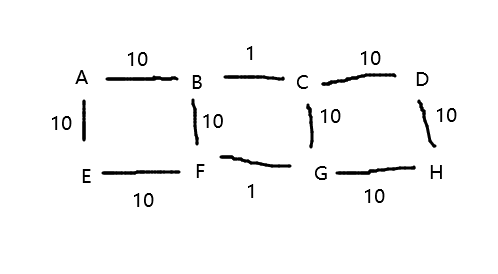
\includegraphics{p1ce.png}
\end{figure}

When edge BC and FG are cut, the weight of the two spanning trees are 30 and 30.\\
Connecting either BC or FG gives a final weight of 30+30+1=61.\\
However, we can see that a less heavy spanning tree can be made using AB, BC, CD, DH, HG, GF, FE. Which the weight is 10+1+10+10+10+1+10=52.\\
\\ \hspace*{\fill} \\
2. \\
This algorithm works because since we know that if edge e is the heaviest edge in a cycle C in the graph G, it cannot be in the MST.\\
Therefore, by deleting all possible heavy edges in cycle, we get a MST.

\end{problem}



\end{document}

